\subsubsection{Re-Implementing the Hash Table Directly in Python} \label{methods:gpu_accelerating_kmer_counting_jit}
While the CUDA hash table we implemented in the previous section yielded significant speedup when \textit{k}mer counting and much better results than the GPU accelerated version of npstructures' hash table, it required us to dvelve into C++, using CUDA's programming framework and leaving the comforts of Python behind in order to implement.
We therefore explored another possible avenue for implementing such a hash table, this time directly in Python.
CuPy offers more than just a GPU accelerated subset of NumPy's array interface.
Additionally, CuPy allows for custom kernels written directly in Python, to be \textit{jit} (just-in-time) compiled.
By exploiting this, we were able to re-implement our parallel hash table directly in Python using CuPy's jit functionality.
This implementation can be found online at \url{https://github.com/jorgenwh/cupycounter}.

\subsubsection{Assessment}
Again, we used the same benchmark used to assess the CuPy-based npstructures counter and the CUDA hash table (section \ref{methods:initial_testing:assessment}), to also assess the CuPy JIT (just-in-time) compiled implementation where we wrote custom kernels to get near-identical behaviour and performance as the CUDA hash table, all directly in Python.
The benchmark yielded the following results:
\begin{table}[H]
\begin{center}
\begin{tabular}{lllll}
\multicolumn{1}{l|}{\textbf{Backend}} & \multicolumn{1}{l}{\textbf{Counting time (seconds)}} &  \\ \cline{1-2}
\multicolumn{1}{l|}{NumPy} & \multicolumn{1}{l}{234.7} &  \\
\multicolumn{1}{l|}{CuPy} & \multicolumn{1}{l}{24.31} &  \\
\multicolumn{1}{l|}{CUDA} & \multicolumn{1}{l}{2.94} &  \\
\multicolumn{1}{l|}{CuPy JIT} & \multicolumn{1}{l}{2.99} &  \\
\end{tabular}
\end{center}
\caption{
  The total time spent counting \textit{k}mers using the just-in-time compiled kernels written directly in Python using CuPy's custom kernel support.
  NumPy, CuPy and CUDA refers to the previous benchmark results from section \ref{methods:initial_testing:assessment} and \ref{methods:gpu_accelerating_kmer_counting:assessment}.
}
\label{methods:gpu_accelerating_kmer_counting_jit:tables:benchmark}
\end{table}

\begin{figure}[H]
\hspace*{7em}
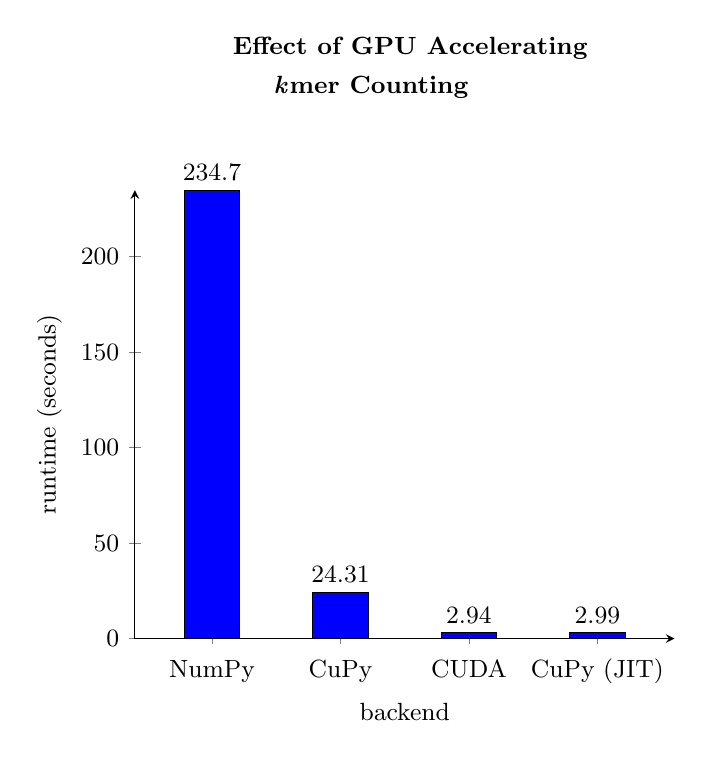
\begin{tikzpicture}[font=\small]
  \pgfplotsset{
    compat=newest,
    xlabel near ticks,
    ylabel near ticks
  }
  \pgfplotsset{compat=1.11,
      /pgfplots/ybar legend/.style={
      /pgfplots/legend image code/.code={%
         \draw[##1,/tikz/.cd,yshift=-0.25em]
          (0cm,0cm) rectangle (3pt,0.8em);},
     },
  }
  \node at(3.5,7.5)(){\textbf{Effect of GPU Accelerating}};
  \node at(3,7)(){\textbf{\textit{k}mer Counting}};
 
\begin{axis} [
  ylabel={runtime (seconds)},
  xlabel={backend},
  ybar,
  bar width=20pt,
  ymin=0,
  xtick=data,
  axis x line=bottom,
  axis y line=left,
  enlarge x limits=.2,
  symbolic x coords={NumPy, CuPy, CUDA, CuPy (JIT)},
  xticklabel style={anchor=base, yshift=-\baselineskip},
  /pgf/number format/.cd,fixed,precision=3,
  nodes near coords={\small\pgfmathprintnumber{\pgfplotspointmeta}},
  legend style={anchor=west},
]

\addplot[fill=blue] coordinates {
    (NumPy, 234.7)
    (CuPy, 24.31)
    (CUDA, 2.94)
    (CuPy (JIT), 2.99)
};
\end{axis}
\end{tikzpicture}
\caption{
  Elapsed time counting the occurences of 50 million unique \textit{k}mers in a set of 20 million reads, each of 150 bases.
}
\label{methods:gpu_accelerating_kmer_counting_jit:figures:benchmark}
\end{figure}

As can be seen in table \ref{methods:gpu_accelerating_kmer_counting_jit:tables:benchmark}, the CuPy just-in-time compiled method of GPU accelerating \textit{k}mer counting resulted in (close to) identical performance as the CUDA hash table implementation, all in spite of being implemented directly in Python using CuPy's custom kernel support.
The memory usage using the CuPy just-in-time compiled solution was also practically identical to the CUDA hash table's.
